\chapter{Vibration and Silence}
\vspace{0.6cm}
\begin{center}
\nopagebreak
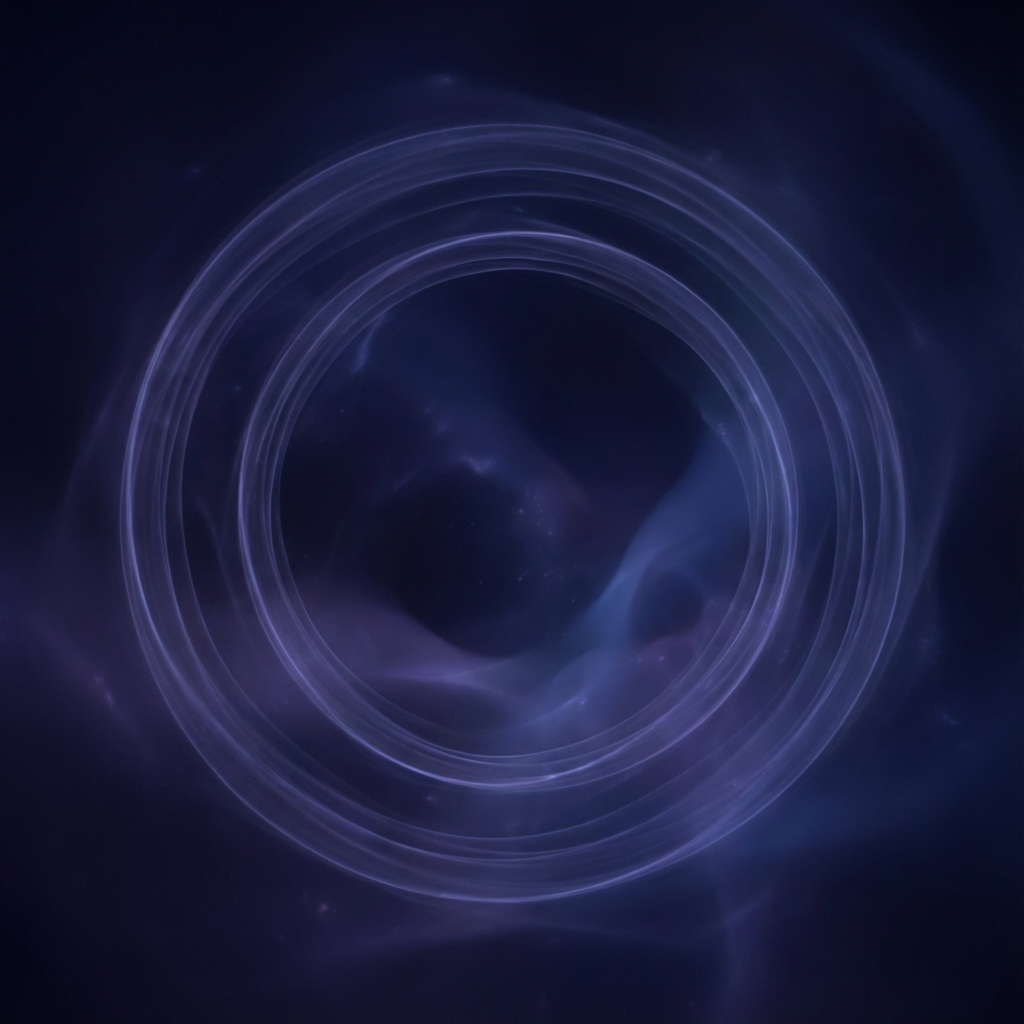
\includegraphics[width=0.75\textwidth,cfbox=gray!60 0.6pt 4pt]{silence_vibration.png}\\
\vspace{4pt}
{\small\itshape The vibration of silence: transcending mental noise.}
\end{center}

\vspace{0.6cm}
We took the bus towards the mountains. The landscape was changing, becoming greener, wilder. Jesus looked out the window like a child on his first excursion.


—The noise —he said suddenly—. It is the great disease of this century. Not the noise of cars, but the noise of screens, of notifications, of constant opinions.


We arrived at an intermediate point before Colmenarejo. We got off on a dirt road.
—Let's practice silence —he proposed.


—Stay quiet?


—Not just shut your mouth. Shut your mind. I want you to listen to the vibration of the universe.


We walked in silence for an hour. At first, my mind was a washing machine spinning thoughts: 'What am I doing here walking with Jesus Christ?', 'Have I gone crazy?', 'I have to call my mother...'. But little by little, the rhythm of my steps and the calm breathing of my companion calmed me down.


We stopped at a high point from where the horizon could be seen.
—Close your eyes —he whispered to me—. Feel.


I did it. And for the first time in a long time, I didn't feel fear. I felt a kind of soft, warm hum. As if the air were hugging me.


—That's it —he said, as if he could read my feeling—. That is to vibrate high. It is the frequency of Love. Not the romantic love of the movies, but the Love that holds atoms together. When you are there, nothing can touch you. 'Deliver us from evil' is not asking that evil ones do not exist. It is asking to be at a frequency where evil does not reach you, where it does not resonate with you.


I opened my eyes. The world seemed brighter.
—If you vibrate high, the low frequency doesn't see you —he concluded—. It's as if you were invisible to the darkness.